
\documentclass [11pt]{report}

\usepackage{fancyhdr}
\usepackage [french]{babel}

\usepackage[utf8]{inputenc}
\usepackage[T1]{fontenc}
\usepackage{textcomp}
\usepackage{graphicx}
\usepackage{titlepic}
\usepackage{boxedminipage}
\usepackage{listings}
\usepackage{minitoc}
\usepackage{footmisc}
\usepackage{color}
\usepackage{graphicx}

\usepackage{eso-pic}

\makeatletter
\newlength\@tempdim@x
\newlength\@tempdim@y
% structure des commandes :
%   #1 = deplacement selon x
%   #2 = deplacement selon y
%   #3 = texte à mettre
\newcommand\AtUpperLeftCorner[3]{%
\begingroup
\@tempdim@x=0cm
\@tempdim@y=\paperheight
\advance\@tempdim@x#1
\advance\@tempdim@y-#2
\put(\LenToUnit{\@tempdim@x},\LenToUnit{\@tempdim@y}){#3}%
\endgroup
}
\newcommand\AtUpperRightCorner[3]{%
\begingroup
\@tempdim@x=\paperwidth
\@tempdim@y=\paperheight
\advance\@tempdim@x-#1
\advance\@tempdim@y-#2
\put(\LenToUnit{\@tempdim@x},\LenToUnit{\@tempdim@y}){#3}%
\endgroup
}
\newcommand\AtLowerLeftCorner[3]{%
\begingroup
\@tempdim@x=0cm
\@tempdim@y=0cm
\advance\@tempdim@x#1
\advance\@tempdim@y#2
\put(\LenToUnit{\@tempdim@x},\LenToUnit{\@tempdim@y}){#3}%
\endgroup
}
\newcommand\AtLowerRightCorner[3]{%
\begingroup
\@tempdim@x=\paperwidth
\@tempdim@y=0cm
\advance\@tempdim@x-#1
\advance\@tempdim@y#2
\put(\LenToUnit{\@tempdim@x},\LenToUnit{\@tempdim@y}){#3}%
\endgroup
}
% ajout de texte ou d'images en haut à gauche, en haut à droite, etc.
\AddToShipoutPicture{%
\AtLowerRightCorner{3cm}{1cm}{
\includegraphics[scale=0.20]{images/LogoGroupe.png}}% image en bas à droite
}
\makeatother

\pagestyle{fancy}



\title{
	
\includegraphics[scale=0.43]{images/Logojeu.png}
	 \\\vspace{20mm}
	\textbf{\Huge \itshape Cahier des charges }
	}




\author{ \\\vspace{2mm}
	Thibault Gdalia\\\vspace{2mm}
	Florent Youinou\\\vspace{2mm}
	Mathilde Laplaze\\\vspace{30mm}
	}


\date{17 janvier 2014}


\begin{document}

\renewcommand{\baselinestretch}{0.001}
\maketitle
\tableofcontents

\newpage


\textbf{{\Huge Introduction}}\\
\\
\\
		\indent Pour notre première année à EPITA (année de Sup), nous avons un projet libre à développer par petit groupe de 3personnes. Nous avons donc formé notre groupe : la Team Girafe, qui vous sera présenté plus loin. Ce projet devant exclusivement être codé en C\# ou en Caml, nous avons décidé de créer un jeu vidéo (on 		aime l'originalité de l'idée). Et il faut le reconnaitre, avoir l'opportunité de créer un jeux vidéo dès sa première année est une chance que nous offre EPITA. En effet, réaliser un jeux nous permet d'apprendre de façon ludique et nous donne vraiment envie d'essayer d'exploiter le potentiel du C\# (même si cela ne reste qu'une petite partie 		de ses capacités vu son étendue).\\

		\indent Travailler en groupe est un un point important et parfois même difficile. Il faut donc que l'ensemble des membres soit motivés ne serait-ce qu'à l'idée de faire un jeux. Naturellement, il faut aussi une bonne entente au sein du groupe, puisque nous passerons beaucoup de temps ensemble, cela contribuera grandement à la 			réussite de ce projet. C'est pourquoi la question principale qui s'est posée en tant qu'entretien d'entrée dans le groupe à été : êtes-vous motivé ?\\\\
		\indent Ainsi, tout au long de ce cahier des charges, vous allez pouvoir comprendre qui nous-sommes, ce que nous comptons faire, mais aussi comment nous comptons le faire. Tout en espérant qu'elle vous plaira : Bonne lecture.
		
\chapter {Pr\'esentations}

	\section{ L'\'equipe }

		La Team Girafe est  un groupe constitué de trois personnes : Mathilde Laplaze alias "Mattou", la seule fille du groupe, Florent Youinou alias "T4ze" et Thibault Gdalia alias "Skeat", le chef de ce projet. Retenez bien ces pseudos car dans le reste de ce cahier des charges nous n'utiliserons plus nos 		noms et pr\'enoms. Nous sommes r\'epartie sur deux classes : la SUPB2 et la SUPD2. \\
		\indent  Nous savons qu'il n'est pas impossible de travailler entre \'el\`eves de classes diff\'erentes. En effet, Skeat a déjà vecu cette expérience l'année dernière. Le groupe a \'et\'e form\'e en fonction des affinit\'es, ainsi que des comp\'etences de chacun que nous avons pu observer durant le premier semestre. 		Pour une meilleure ambiance dans l'\'equipe, et pour avoir un bon rythme de travail, le groupe s'est constitué de membres qui ont la volont\'e de travailler. 
	
	
	
	\newpage

	\section { Les Membres }
		\subsection {Mathilde "Mattou" Laplaze}
			Mattou ou Mathilde Laplaze J'ai 18 ans, et je n'ai jamais touché à l'informatique avant mon entrée a EPITA (la honte).C'est biensur la majorité de la gente masculine qui m'a poussée à me tourner vers ce secteur.\\
			\indent Plus sérieusement,l'idée d'être capable de créer et développer mes propres projets informatiques m'a donné envie et c'est un secteur très prometteur.J'ai eu beaucoup de mal trouver un groupe pour le projet, du fait que je ne suis qu'une fille et que les garçons aux pensées innocentes ne courent pas les rues.Ou 			d'autres s'imaginent qu'une fille a moins de capacité qu'eux. Heureusement, je suis tombée sur ce groupe, avec lequel je ne me fais pas de soucis.La seule difficulté est que j'habite en Picardie, et le temps de transport me laisse très peu de temps libre pour participer au projet.\\\vspace{10mm}
	
		
	

		\subsection {Florent "T4ze" Youinou}
			T4ze, c’est moi. \'Etant fils d’ingénieur en informatique, ma passion me vient de mon père et contrairement aux enfants de mon âge, je n’ai jamais été un grand fan des jeux vidéo. Ainsi pendant que les autres s’amusaient sur leur console, moi je bidouillais sur mon ordinateur. J’ai donc commencé tôt à coder. Connaissant mes ambitions je me suis très vite investi dans les études qui me permettraient d’y accéder. Par conséquent, je considérais que les autres matières étaient totalement inutiles et me faisaient perdre mon temps. J’ai donc passé un bac S SI (Science de l’Ingénieur) avec la spé ISN. J’adore apprendre et écouter les suggestions construites de personnes extérieurs.\\
			\indent Mais l’idée de vivre accroché à un siège devant un écran ne donne pas envie, heureusement j’ai d’autres passions pour me changer les idées. En effet, je fais beaucoup de sport, je sors souvent et ma plus grande source d’inspiration pour coder me vient des films que je regarde.\\
\vspace{10mm}

	
		
		
		\subsection {Thibault "Skeat" Gdalia}

			Moi c'est Skeat, je suis en SUP a EPITA pour la deuxi\`eme fois (oui j'ai redoubl\'e),  c'est donc mon deuxi\`eme projet, l'ann\'ee derni\`ere au sein du groupe DAMNIT. Cette ann\'ee je suis toujours motiv\'e pour travailler en groupe, et accro\^itre mes comp\'etences en C\# . \\
			 \indent  Avant de rentrer à EPITA, j'ai fait une terminal S Sciences de l'Ing\'enieur, c'est là que j'ai découvert la programmation, ça m'a tout de suite beaucoup plus. J'ai commenc\'e à coder en Visual Basic en cours au lyc\'ee puis je me suis tourn\'e vers le C++, mais cette fois tout seul.\\
		 	\indent Je n'ai jamais \'et\'e un grand fan de jeu vid\'eo, j'ai toujours pr\'ef\'er\'e faire du sport ou sortir faire la f\^ete (donc rien a voir avec un GEEK). L'ann\'ee derni\`ere, je n'ai pas valid\'e mon ann\'ee car je suis arriv\'e avec trop de lacunes, mais cette ann\'ee va \^etre une autre histoire, c'est pour cela que j'ai choisi  			de faire parti de ce groupe qui est tr\`es motiv\'e et travailleur. De plus je connais tr\`es bien TiNyDGZz avec qui j'ai travaill\'e l'ann\'ee derni\`ere, et je sais que l'on peut compter sur lui, ce qui est essentiel dans un travail de groupe.\\\vspace{10mm}
	
	

\chapter{Principe et histoire du jeu}

		\indent Nous sommes partis sur un jeu en 2D bas\'e sur un principe tr\`es connu, que l'on retrouve dans Jetpack ou encore Badland, tout en y apportant notre touche personnel. Le personnage doit parcourir les différentes maps du jeu, en évitant les nombreux obstacles se trouvant sur son chemin. Afin que le jeu est un peu plus 		d'intérêt pour le joueur, les maps devront être debloquées les unes à la suite des autres, et deviendront de plus en plus dur, avec de nouveaux obstacles.\\

		\indent Le joueur ne pourra pas déplacer son personnage comme il le souhaite (sinon c'est trop simple..). Il ne pourra que lui faire effectuer un bond en appuyant sur la touche espace (jusque la rien d'impressionnant). \`A chaque fois que le joueur touche un obstacle il est ralenti et doit changer sa trajectoire. Mais en plus de cela, il 	devra manger les bonbons qui se trouvent sur son parcours si il veut faire remonter sa barre d'energie. Et mieux vaux qu'il le veuille puisque lorsque le joueur effectue un bond, son personnage consomme de l'énergie et donc sans énergie : pas de bon. Pour regagner son énergie, il peut aussi patienter le temps que la barre se régénère 		(et prier pour qu'il n'y ai pas d'obstacle). La partie est perdue si le personnage sort de l'écran par la gauche, par exemple en étant bloqué par un obstacle. Et au contraire, si il parvient jusqu'au bout de la map, la partie est remportée et on passe à la map suivante.

\newpage 


\chapter {Partage du travail}
\begin{center}
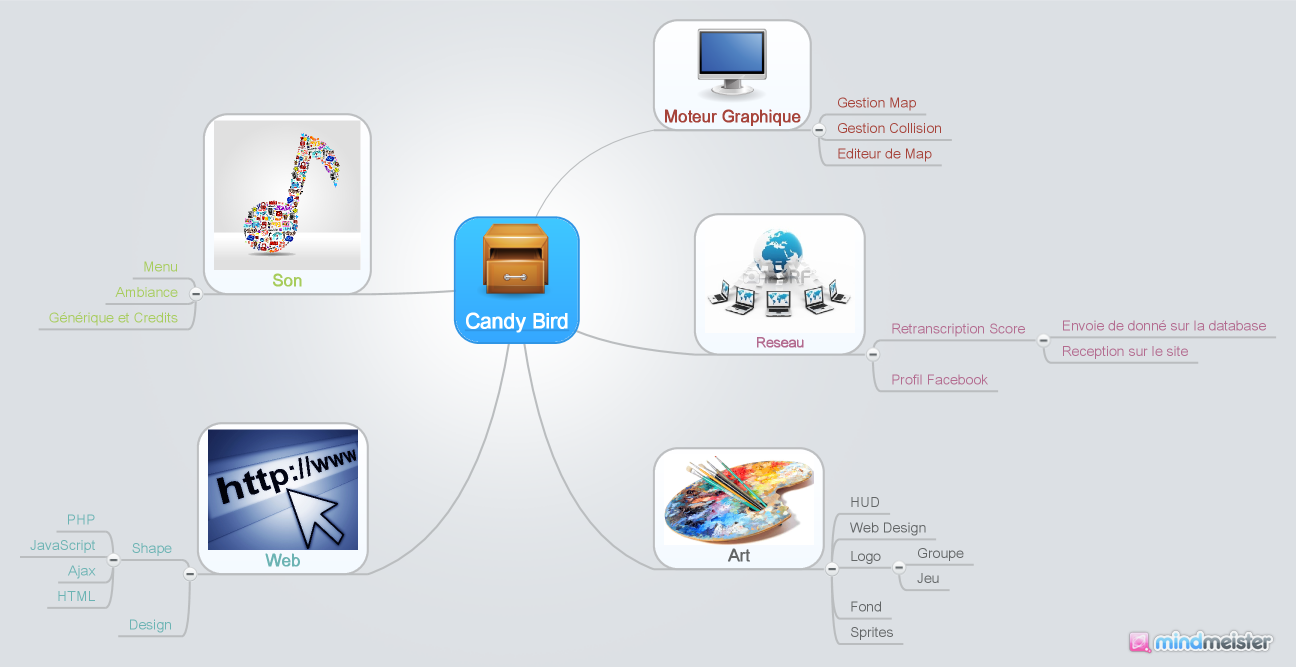
\includegraphics[scale=0.3]{images/Candy_Bird.png}
\end{center}

\newpage 

	


	\section{Graphismes}
		\subsection {Logo}
			\paragraph{Jeu}
				L'idée de ce logo provient du célèbre jeu CandyCrush, et sa couleur Orangée/Marron s'inspire des sodas. Les reflets clairs et les bulles présents un peu partout dans le titre rappellent le côté sucré d'un bonbon et annoncent ainsi en quelque sorte l'idée du jeux (un oiseau gourmand qui doit avaler des bonbons pour 				avoir des forces). \\

			\paragraph{Groupe Cf. Bas de page}
				Le logo de groupe quant à lui a été décidé un peu au hasard. En effet, un jour Skeat a vu un Flashcode et se s'est demandé pourquoi ne pas en faire le logo du groupe. Lorsque vous flashez le flashcode (Logique non ?) il vous amènera directement sur le site internet du projet, ce qui nous permet de nous 				faire connaitre implicitement. Pour ne pas avoir un simple flashcode noir et blanc, nous avons cherché à le personaliser et c'est ainsi que s'est crée notre logo. Pour rester dans les tons du jeux, sa couleur bleue a été choisie pour rappeler la salopette bleue du petit oiseau principal !\\\vspace{5mm}

		\subsection {Fonds, Obstacles et Personnage(s)}
	 		Les fonds qui défilent ainsi que les obstacles sont installés avec une version par défaut mais ils pourront par la suite être modifiés en fonction de la période. Par exemple un thème hiver, été, paques, noel, etc..\\\\\\
 			\indent Pour rester fidèle au nom du jeux, CandyBird, le personnage officiel est donc un oiseau, et plus précisément un houla-houla.
Mais cet animal est loin d'être un oiseau ordinaire. En effet, à cause de la partie inférieure de son corps trop développée, il lui est difficile de voler pres du sol. De plus, c'est un animal gourmand et peu joyeux. Il a besoin d'avaler une grande quantité de sucre pour pouvoir s'envoler.\\
			\indent Cet oiseau, tout comme les fonds, pourra être modifié dans des versions ultérieures du jeux et ainsi se transformer en d'autres espèces.\\\vspace{5mm}



	\section {Moteur Physique}
			Pour ce type de jeu le moteur physique est assez rudimentaire. Nous avons donc décidé de jouer avec les lois de la physique, sinon c'est pas drôle. Pour nous les propriétés physique de notre quotidien ne sont pas assez compliqués, Alors d'une map à l'autre ou en même au cours d'une même map les propriétés 				changeront, ce qui rendra le jeu un peu plus dure et amusant. Ainsi, la vitesse de l'oiseau et la gravité ne cesseront de changer. Toujours dans le but de rendre le jeu plus divertissant,le joueur n'aura pas la possibilité de faire descendre son personnage, ni de décaler l'oiseau sur la droite ou sur la gauche, il ne pourra qu'attendre le meilleur 	moment pour lui faire faire un bond.\\\vspace{2mm}


\section {Multijoueur}
		Une partie du jeu sera consacrée au réseau multi-joueurs. CandyBird permettra, en effet, de jouer en ligne avec un partenaire (des versions ultérieures du jeu permettront peut-être d'augmenter le nombre de joueurs). Chaque joueur de la partie verra alors son adversaire avancer sur la map et sera obligé d'arriver avant lui et de ne pas se faire distancer s’il veut gagner la partie. Certains bonus seront accessibles afin de cacher une partie de l'ecran de l'adversaire, ou de le destabiliser. Le mode multi-joueurs sera accessible depuis le menu principal. Ce réseau pourra fonctionner en wifi ou par câble Ethernet. \\ \vspace{5mm}



	\section {Réseaux}
		Afin de rendre le jeux plus interessant d'un point de vue social, l'idée nous est venu de mettre en place un système de classement. En ouvrant le jeux il nous sera donc possible de se connecter (à un compte créé auparavant) ou de jouer localement. Si l'on se connecte, en fin de partie notre score sera automatiquement envoyé sur le site officiel du jeux et s'affichera dans la catégorie classement. Cela permettra de comparer son score avec celui d'un ami, ou tout simplement de voir notre niveau par rapport à tous les joueurs.\\\vspace{3mm}


	




	\section {Menu}
		Un menu facilitera l'agencement des différents états du jeux. Dans le menu principale, il sera possible de se connecter à son compte à la seule condition, que le joueur ai préalablement créer son profil via notre site internet ou directement depuis le jeux. Il sera aussi possible de naviguer depuis cle menu à travers les options du jeux 		où l'on aura par exemple le choix entre activer ou désactiver le son du jeu ou encore régler la résolution du jeux afin t'optimiser l'affichage en fonction de son ordinateur. \`A tout moment, l'utilisateur pourra bien évidement commencer une nouvelle partie. \\
		\indent Durant une partie un menu pause sera disponible pour ne pas avoir à quitter entièrement le jeux, ou à perdre la partie losque l'on doit faire quelque chose entre temps. Dans ce menu, le joueur pourra : reprendre la partie, revenir au menu principal ou encore quitter le jeu.\\\vspace{5mm}


	\section {Communication}
		Pour permettre au jeux de se faire conna\^itre, et pour suivre son \'evolution, un site web sera mis en place. Une grosse partie du site sera dédiée aux nouveautés du jeux, aux présentations ainsi qu'aux rapports de soutenances. Une partie photo regroupera quelques clichés de nous travaillant sur le projet et des screen-shot du 		jeux. Un formulaire de contact sera disponible afin de nous faire part d'idée d'am\'eliorations, de bug, ou de tout commentaire relatif au jeux. Quand la gestion réseau sera opérationnelle, nous mettrons aussi en place une page dédiée au classement des joueurs.
	\\
	\\
	 \indent De plus, une page facebook sera ouverte à l'effigie de notre jeu. Car nous savons qu'il est plus simple de toucher un maximum de personnes par l'intermédiaire de ce réseau social. Nous y mettrons l'ensemble de nos actualités, les nouveautés sur le jeu, des images de notre travail afin d'interpeler les internautes. De plus, il y sera 		très simple de nous contacter quelqu'en soit la raison.\\\vspace{5mm}

	\section {\'Editeur de Maps}
		Nous avons décidé de faire les maps dans des fichiers externes, sous formes de tableaux en associant des caractères spécifiques à chaque élément du décors (par exemple un 1 sera un carré rouge). Comme que nous n'avons aucune envie d'écrire toutes les maps à la main (nous pouvons perdre notre temps autrement), nous 		allons créer un éditeur de maps, tout d'abord pour nous, et une fois que nous aurons une interface graphique digne de notre jeu, il sera par la suite intégré au jeu, afin le joueur pourra lui même créer des niveaux et pourquoi pas les partager avec les autres joueurs pour les mettre au défis, ce qui nous permettra d'allonger la durée de 		vie du jeu.\\\vspace{5mm}


\newpage
	\section {Son}
		Un jeux, c'est bien, mais avec du son c'est mieux ! Nous allons utiliser une extension de XNA, Xact, qui nous permettra de g\'erer une biblioth\`eque de sons dans le jeux. Cette biblioth\`eque nous permettra d'am\'eliorer nos \'ev\'enements avec des musiques d'ambiances (sound sur Xact) et des effets sonores lors des actions du 		joueur , sera accompagné d'un sound effect. Ainsi chaque événement lors d'une partie tel que les bons de l'oiseau ou lors d'une collision entre l'oiseau et un élément du décor, toutes les maps auront donc leur propre ambiance, par contre il n'y aura qu'une seule et même légère musique dans les menus. L'ensemble des sons seront récupérés sur internet car nous n'avons malheureusement pas de musiciens dans notre groupe (nous feront avec ce que nous trouverons). Puisque la musique n'est qu'une feature du jeux, il faut limiter son temps de recherche, nous ne seront donc que deux à travailler sur cette partie.\\\vspace{5mm}

	\section{Repartitions}
		\subsection{Tâches}
			\begin{tabular}{| l |*{3} {c|}}
				\hline
				Themes & Mathilde & Florent & Thibault \\
				\hline
				Son & Responsable & & Aide \\
				\hline
				Multi-joueur & & Responsable & Aide \\
				\hline
				Moteur Physique & Aide & Aide & Responsable\\
				\hline
				Editeur de Map &   & Aide & Responsable\\
				\hline
				Site Internet & & Responsable & \\
				\hline
				Graphisme & Responsable & & \\
				\hline
				
			\end{tabular}\\\vspace{3mm}


		\subsection{Soutenances}
			\begin{tabular}{| l | * {3}{c|}}
				\hline
		 		& Soutenance 1 & Soutenance 2 & Soutenance 3 \\
				\hline
				Moteur Physique & 50\% & 75\% & 100\% \\
				\hline
				 Graphisme & 50\% & 80\% & 100\% \\
				\hline
				Réseaux & 0\% & 50\% & 100\% \\
				\hline
				Site internet & 50\% & 100\%  & 100\%  \\
	          			 \hline
				Son & 50\% & 80\% & 100\% \\
				\hline
				\'Editeur de map & 50\% & 100\% & 100\% \\
				\hline
			\end{tabular}\\\vspace{4mm}


\chapter {Ressources utilisées}
	\section {Logiciels}

	Pour ce projet nous utiliserons plusieurs logiciels afin de programmer les différentes parties :\\

	- Notepad++ : Le site internet ainsi que les premières maps ont quasiment toutes été entierement codés à la main via cet éditeur de texte.\\\\\indent
	- Wamp : Pour pouvoir créer et tester le site en local.\\\\\indent
	- Visual Studio 2010 (avec XNA) : Afin de réaliser notre jeux en c\#, nous avons utilisé Visual Studio.\\\\\indent
	- Photoshop CS6 : La plupart des graphismes ont été réalisés à l'aide de Photoshop.\\\\\indent
	- TeXWork : Parce que écrire du \LaTeX sur le bloc note c'est pas simple.\\\vspace{8mm}



	\section {Autres}

	Pour apprendre/comprendre les différents langages de programmations dont nous nécessitions, nous avons utilisé de nombreux tutoriels, dont nous avons besoin, nous avons également chercher sur internet comment utilisé les logiciels. Et comme la plupart du temps quand on a un probleme, on est pas le seul, les forums nous ont permis de corriger des bugs ou même améliorer notre code.


\chapter {Budget pour le projet}
	Nous avons fait une petite prévisions de nos dépenses pour ce projet :\\\\

				\begin{tabular}{|l|c|}
				\hline
		 		 & Prix \\
				\hline
				Années a \'Epita (x4) & 22 800 € \\
				\hline
				Ordinateur (x3) & 4 085 €  \\
				\hline
				Nom de Domaine et Hébergement &  15€ \\
				\hline
				T-shirts & 80€ \\
				\hline
				Tablettes de chocolat & 200€ \\
				\hline
				Pizzas et Kebabs & 420€  \\
				\hline
				Bières  & 420€   \\
	          			 \hline
				Soirée d'après soutenance (x3) & 1200€\\
				\hline 
				Cadeau pour que le jury nous aime & 42€ \\
				\hline
				Total & beaucoup trop cher \\
				\hline
				
			\end{tabular}
\newpage
\textbf{{\Huge Conclusion}}\\
\\
\\\indent	Notre projet est donc basé sur un jeu de style Jetpack en 2D et représente un assez grand défi pour nous. C’est pourquoi nous sommes motivé et prêts à réaliser ce jeu entièrement et pourquoi pas y rajouter quelques nouveautés imprévues. Le mode solo permettra donc de se défier sois même et une fois connecté , le joueur pourra se défier a d’autres joueurs et les scores seront transmis sur le site web de notre projet. Le travail personnel et collectif que nous devons fournir tend à enrichir notre propre expérience,e et nous apporter un certain nombre de comp\'etences.

\end {document}